\label{Sec:OptimalVaccinePolicies}
%!TEX root = main.tex
According to dynamics in \Cref{model1,eqn:model1_counters}, we modulate the
vaccination rate by a time-dependent control signal $u_V(t)$ to
achieve an imposed vaccine coverage. That is, according to the components $S$,
$V$, $X$ of \Cref{model1,eqn:model1_counters}, we modulate the
vaccination rate $\lambda_V$ by an additive control $u_V(t)$. Thus, we modify
components equations related with $S$, $V$, $X$ as
\begin{equation}
    \label{eqn:counter}
    \begin{aligned}
        S'(t) & =
        \mu \bar{N} - \frac{\beta_S I_S + \beta_AI_A}{\bar{N}}S
        - (\mu + (\lambda_V + u_V(t)) S
        + \delta_V V + \delta_R R
        \\
        V'(t) &=
        (\lambda_V + u_V(t)) S-(1-\epsilon)
        \frac{\beta_S I_S + \beta_A I_A}{\bar{N}}V
        - (\mu+\delta_V) V
        \\
        X'(t) &=
        (\lambda_V + u_V(t)) (S + E + I_A + R).
    \end{aligned}
\end{equation}
In order to assure solution of our controlled model we
consider the functional space
$$
\mathcal{U}[0:T]:=
\left\{
u_V: [0, T] \to \mathbb{R},
\text{ such that $u_V(\cdot)$ bounded and piecewise continuous}
\right\}.
$$
Let ${x(t):= (S,E,I_S,I_A,R,D,V,X)^{\top}(t)}$
and control signal $u_V(\cdot)\in \mathcal{U}[0, T]$.
Following the guidelines of
WHO-SAGE modeling questions \cite{sage2020},
we quantify the burden of COVID-19, according
to the Disability-Adjusted Life Year (DALY) unit. Thus adapting the WHO
definition of DALY \cite{WhoDALY}, we optimize the number of years of life lost
with a vaccination policy. In other words, we calculate a minimum of
the penalization functional
\begin{align}
    \label{eqn:cost_functional}
    J(u_V) =
    a_D ( D(T) - D(0)) +
    a_S (Y_{I_S}(T) - Y_{I_S}(0)).
\end{align}
Here, $a_S$ and $a_D$ are parameters related with the units definition of the
Years of Life Lost (YLL) due to premature mortality and the Years Lost due to
Disability (YLD). We estimate $a_D$ as the mean life expectancy at the age of
death, and according to Mexico City+Mexico state data, we handle
$a_D = \SI{7.5}{years}$.
Parameter $a_S$ is the product of a disability weight (DW) and the average
duration of cases until remission or death in years, that is,
$
a_S = DW \times \alpha_S^{-1}
$.
Here we postulate the disability weight as the arithmetic average of disability
weight regarding comorbidities reported in \cite{Jo2020}. Thus, our simulations
employ $a_S= \SI{0.008418473}{years}$.
%
Thus, functional $J$ penalizes the pandemic burden\textemdash in Years
of Life Lost\textemdash due to mortality or disability. We display in
\Cref{tbl:ocp_parameters_description} parameters regarding with the optimal
controlled model.

Since we aim to simulate vaccination policies contra factual scenarios
following the SAGE modeling guidelines reported in \cite{sage2020},
we impose the vaccination counter state's horizon time condition $X(T)$
\begin{equation}
    \label{eqn:coverage_constrain}
    \begin{aligned}
        x(T) &=
        (\cdot, \cdot, \cdot, \cdot, \cdot, X(T))^{\top}
        \in \Omega,
        \\
        X(T)
        &= x_{cover age},
        \\
        x_{coverage}
        & \in
        \left \{
        \text{Low(0.2)},\text{Mid(0.5)}
        \right \} .
    \end{aligned}
\end{equation}
Thus, given the time horizon $T$, we set the last fraction of
vaccinated populations corresponds to 20\% or 50\%, and the rest of
final states as free. We also impose the path constraint
\begin{equation}
    \label{eqn:path_constrain}
    \Phi(x,t):= \kappa I_S(t) \leq B,
    \qquad \forall t \in [0, T],
\end{equation}
to ensure that critical symptomatic cases
will not overload healthcare services. Here $\kappa$
denotes hospitalization rate, and $B$ is the load capacity of a
health system. We illustrate the main ideas of the above discussion
in \Cref{Fig:SchemeModel_opt}.
\begin{figure}[h!]
    \centering
    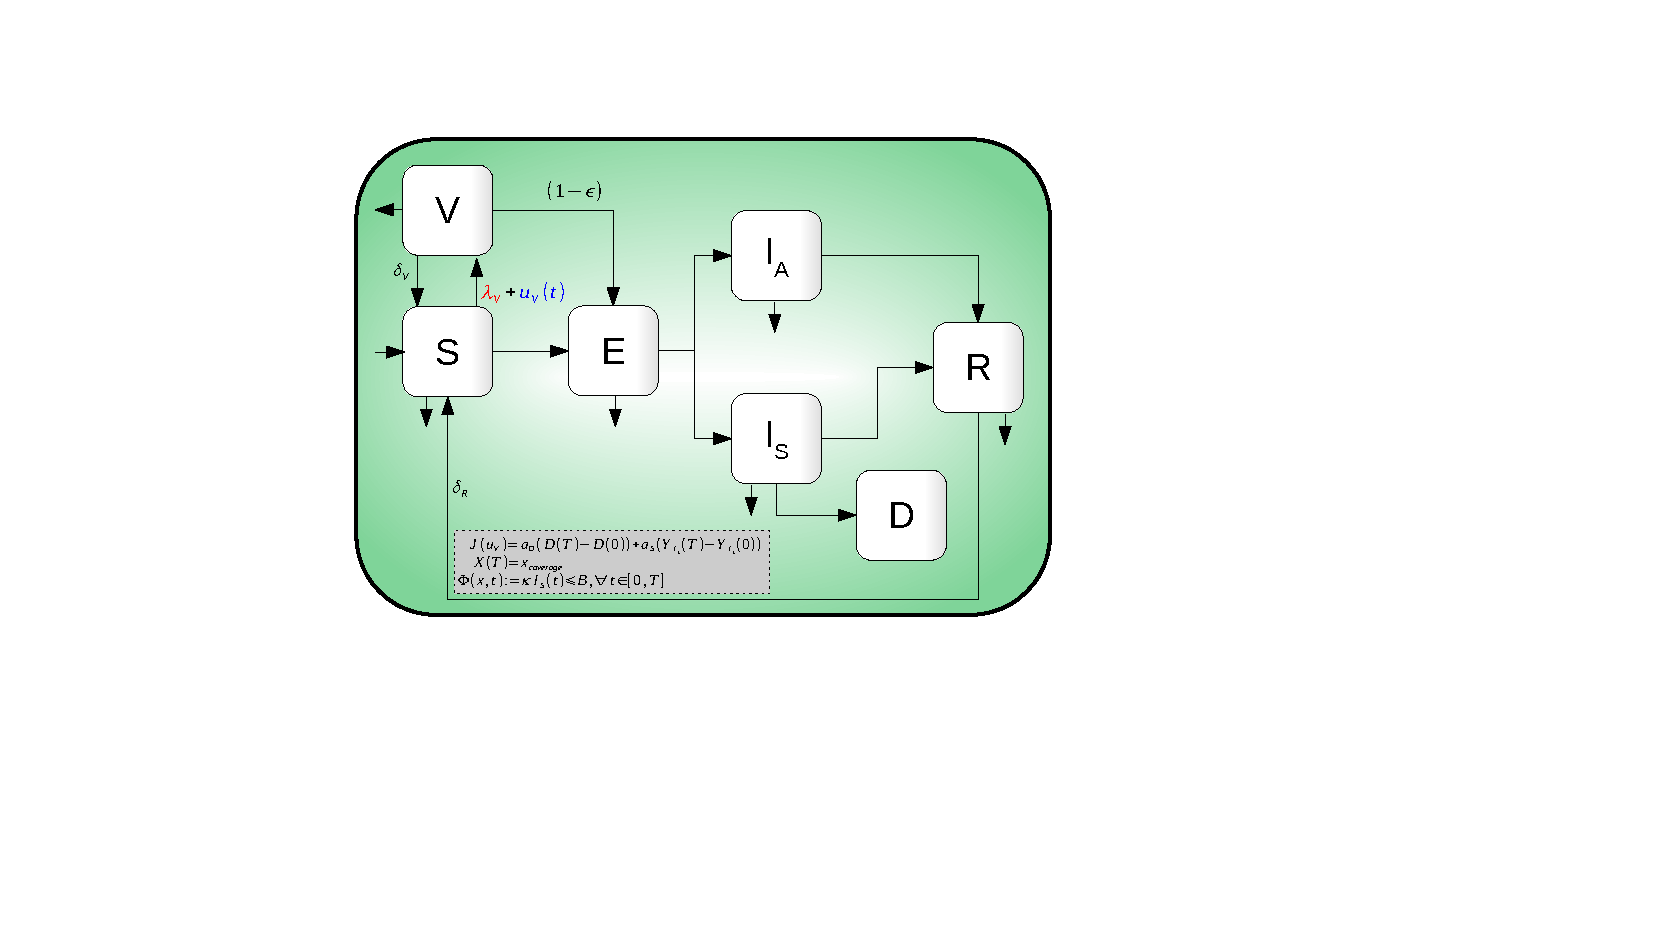
\includegraphics[scale = 1]{SchemeModel_0211_v4.pdf}
    \caption{Compartmental diagram of COVID-19 transmission dynamics which
        including optimal vaccination dynamics, penalization and path
        constraint.}
    \label{Fig:SchemeModel_opt}
\end{figure}

Given a fixed time horizon and vaccine with efficacy $\epsilon$,
we estimate the constant vaccination rate $\lambda_V$ as the solution of
\Cref{eqn:lambda_base}.
That is, $\lambda_V$ estimates the constant rate
to cover\textemdash with a vaccine dose per individual\textemdash
population fraction $x_{coverage}$ in time horizon $T$.
Thus, according to this vaccination rate, we postulate a policy $u_V$ that
modulates vaccination rate according to $\lambda_V$ as a baseline.

Then, optimal vaccination amplifies or attenuates this estimated baseline
$\lambda_V$ in a interval $[\lambda_V^{\min}, \lambda_V^{\max}]$
to optimize functional $J(\cdot)$\textemdash minimizing
symptomatic, death reported cases and optimizing resources.

Our aim is minimize the cost functional
\eqref{eqn:cost_functional}\textemdash over an appropriated
space\textemdash subject to the dynamics in
\Cref{model1,eqn:counter}, boundary conditions related with
\eqref{eqn:coverage_constrain}, and path
constrain \eqref{eqn:path_constrain}.
That is, we seek for vaccination policies $u_V(\cdot)$, that
solve the following optimal control problem (OCP)%
\begin{equation}
    \label{eqn:optimal_control_problem}
    \begin{aligned}
        & \min_{u_V \in \mathcal{U}[0, T]}
        J(u_V) :=
        %\int_0 ^ T
        % a_D D(s) + a_S Y_{I_S}(s) ds
        a_D ( D(T) - D(0)) +
        a_S (Y_{I_S}(T) - Y_{I_S}(0))
        \\
        \text{s.t.} &
        \\
        &f_{\lambda}
        :=
        \frac{\beta_S I_S + \beta_AI_A}{\bar{N}}
        \\
        S'(t)
        &=
        \mu \bar{N} + \delta_V V + \delta_R R
        \\
        &-
        (f_{\lambda} + \mu + \lambda_V +  u_V(t)) S
        \\
        E'(t)
        &=
        f_{\lambda} (S + (1-\epsilon) V)
        - (\mu+\delta_E) E
        \\
        I'_S(t)
        &=p
        \delta_E
        E-(\mu + \alpha_S) I_S
        \\
        I'_A(t)
        &= (1 - p) \delta_E E-(\mu + \alpha_A) I_A
        \\
        R'(t)
        &= (1 - \theta) \alpha_S I_S + \alpha_A I_A
        - (\mu + \delta_R) R
        \\
        D'(t)&=
        \theta \alpha_S I_S
        \\
        V'(t)&=
        (\lambda_V + u_V(t)) S -
        \left(
        (1 -\epsilon) f_{\lambda} V +
        \mu + \delta_V
        \right) V
        \\
        X'(t)&=
        (\lambda_V + u_V(t))(S + E + I_A + R)
        \\
        \\
        S(0) &= S_0, \ E(0) = E_0, \ I_S(0) = I_{S_{0}},
        \\
        I_A(0) &= I_{A_{0}}, \ R(0) = R_0, \ D(0) = D_0,
        \\
        V(0) &= 0, \ X(0) = 0, \ X(T) = x_{coverage},
        \\
        u_V(\cdot) & \in [u_{\min}, u^{\max}],
        \\
        \kappa I_S(t) & \leq B, \quad \forall t \in [0, T],
        \\
        \bar{N}(t) &= S + E + I_S + I_A + R + V.
    \end{aligned}
\end{equation}
\Cref{tbl:ocp_parameters_description} encloses a parameters description
regarding with this controlled
version.

Existence of solution to our (OCP) in
\Cref{eqn:optimal_control_problem} drops in the theory
developed by Francis Clark
\cite[see e.g.][Thm. 23.11]{Clarke2013}. Since our aim is the simulation of
hypothetical scenarios,
we omit here a rigorus proof, instead we refer interested readers to
\cite{Sethi1995,Lenhart2007} and the reference
there in.

\begin{table}[htb]
    \centering
    \begin{tabular}{%
            >{\centering}
            p{0.1\textwidth}
            p{0.38\textwidth}
            p{0.15\textwidth}
            p{0.15\textwidth}
        }
        \toprule
        \textbf{Symbol}
        & \textbf{Description}
        & \textbf{Value}
        & \textbf{Ref}
        \\
        \midrule
        $a_D$
        &
        Penalization weight due to  premature mortality (YLL)
        and estimated from CDMX data
        & $\SI{7.5}{years}$ & \cite{WhoDALY,DataMX}
        \\
        $a_S$
        &
        Penalization weight due to disability (YLD)
        & $\SI{0.008418473}{years}$ & \cite{Jo2020}
        \\
        $x_{coverage}$
        &
        Covering constraint at time horizon $T$
        & & \cite{sage2020}

        \\
        $\kappa$
        &
        Hospitalization rate
        &
        $0.05$
        &
        Estimated
        \\
        $B$
        &
        Health service capacity in number of beds
        normalized by the whole
        population $N$
        &
        $9500$
        &

        \\
        \bottomrule
    \end{tabular}
    \caption{
        Parameters regarding
        controlled version model (OCP) in \Cref{eqn:optimal_control_problem}.
    }
    \label{tbl:ocp_parameters_description}
\end{table}
